%region Sección III
\section{Pruebas y Resultados}
Para la validación de la funcionalidad y el rendimiento del sistema LPR-Sentinel, se ha diseñado un conjunto de pruebas que abarca tanto la evaluación individual de cada módulo como la evaluación del pipeline completo. Las pruebas han sido ejecutadas empleando conjuntos de datos sintéticos generados por los propios módulos MLP-Generator y MLP-Augmentator, así como un pequeño conjunto de imágenes simuladas capturadas en condiciones controladas para verificar la transferencia del aprendizaje. Los resultados presentados en esta sección son representativos del comportamiento observado durante las fases de validación, organizándose en torno a cuatro métricas principales: la calidad y diversidad de los datos sintéticos generados, la eficacia de las transformaciones de aumentación, la precisión y latencia del detector y reconocedor, y el rendimiento integral del pipeline.

\subsection*{Entorno de Desarrollo}
\addcontentsline{toc}{subsection}{Entorno de Desarrollo}
LPR-Sentinel ha sido diseñado para operar en hardware embedido de bajo costo, sin dependencia de GPUs o servidores de alta gama. Como plataforma objetivo se ha seleccionado una Raspberry Pi 4B con 4 GB de memoria RAM y 220 GB de almacenamiento SSD. La razón de su selección, además de su consumo energético inferior a 5 watts en condiciones medias, se debe a que ha sido ampliamente utilizado en aplicaciones de visión artificial embebida, videovigilancia distribuida y sistemas IoT, lo que garantiza su posible escalabilidad y despliegue en entornos reales.

Para maximizar estos recursos disponibles, se instaló el sistema operativo Raspberry Pi OS Lite (64 bits), una versión minimalista de Raspberry OS sin interfaz gráfica. Esta configuración reduce al mínimo la sobrecarga del sistema, dedicando la mayor parte de la capacidad de procesamiento a las tareas de inferencia de los modelos ONNX, aunque esta configuración limita la visualización gráfica en tiempo real. El dispositivo se configura para ser manipulado exclusivamente mediante Security Shell (SSH) a través de una red local, eliminando así la carga asociada a periféricos, aplicaciones en segundo plano o servicios no esenciales. La Figura~\ref{fig_raspberry_setup} muestra el esquema de conexión propuesto.

\begin{figure}[ht]
\centering
% \includegraphics[width=0.6\textwidth]{figures/raspberry_pi_setup.png}
\caption{Configuración del hardware: Raspberry Pi 4B conectada a la red local (Ethernet/WiFi), accesible mediante SSH desde una máquina de desarrollo. Una cámara (USB o módulo CSI) captura imágenes de vehículos, las cuales se procesan localmente. Los resultados se almacenan en en dispositivo local y se visualizan desde el dispositivo remoto mediante la conexión por SSH.}
\label{fig_raspberry_setup}
\end{figure}

Dado que se emplea la versión Lite del sistema operativo, mismo que carece de muchas herramientas de desarrollo preinstaladas, es necesario configurar el entorno manualmente. Entre las herramientas indispensables se incluye la instalación de compiladores y el gestor de paquetes de Python listados en la Tabla \ref{tab_herramientas}.

\begin{table}[h]
\centering
\caption{Herramientas de desarrollo instaladas en la versión Lite del sistema operativo}
\begin{tabular}{|l|p{9cm}|}
\hline
\textbf{Paquete} & \textbf{Descripción} \\ \hline
python3-pip & Gestor de paquetes de Python que permite instalar y administrar librerías desde PyPI. \\ \hline
python3-setuptools & Conjunto de utilidades para empaquetado e instalación de módulos de Python. \\ \hline
build-essential & Metapaquete que incluye compiladores (gcc, g++, make) y herramientas necesarias para compilar dependencias nativas en arquitectura ARM64. \\ \hline
\end{tabular}
\label{tab_herramientas}
\end{table}

\subsection*{Validación del Generador de Matrículas Sintéticas}
\addcontentsline{toc}{subsection}{Validación del Generador de Matrículas Sintéticas}
El módulo MLP-Generator fue evaluado en términos de su capacidad para producir matrículas con las particularidades de cada entidad federativa. Por conveniencia, se generaron 250 matrículas por cada uno de los 32 estados, totalizando 8,000 muestras sintéticas. La validación se realizó con una inspección cualitativa de 1,000 muestras seleccionadas aleatoriamente en conformidad a la normativa. Para cada muestra se verificó la exclusión de las letras problemáticas \quotes{I}, \quotes{Ñ}, \quotes{O} y \quotes{Q}, así como la correcta inclusión del carácter separador \quotes{-} en las posiciones definidas por el formato de cada estado. La Tabla \ref{tab:generation_stats} resume la distribución de matrículas generadas por tipo de formato, donde el formato LLL-NNN-L representa el 93.75\% del total de muestras, mientras que las variantes para Ciudad de México (LNN-LLL) y Guanajuato (LLL-NN-LL) concentran el 6.25\% restante.

\begin{table}[ht]
\centering
\caption{Distribución de matrículas generadas por tipo de formato}
\label{tab:generation_stats}
\begin{tabular}{|c|c|c|}
\hline
\textbf{Formato} & \textbf{Cantidad generada} & \textbf{Porcentaje} \\
\hline
LLL-NNN-L (General) & 7,500 & 93.75\% \\
LNN-LLL (Ciudad de México) & 250 & 3.125\% \\
LLL-NN-LL (Guanajuato) & 250 & 3.125\% \\
\hline
\textbf{Total} & \textbf{8,000} & \textbf{100\%} \\
\hline
\end{tabular}
\end{table}

La fuente tipográfica diseñada reprodujo las proporciones de los caracteres, el color de fondo y las combinaciones oficiales para cada estado (por ejemplo, fondo blanco con tipografía negra para vehículos particulares en la mayoría de los estados). No se detectaron anomalías como caracteres truncados, desbordamientos de los límites de la zona editable o artefactos de renderizado que comprometieran la legibilidad. La Figura \ref{fig:synthetic_samples} muestra una selección de matrículas sintéticas generadas para diferentes estados, respetando las restricciones de rangos y números de serie válidos.

\begin{figure}[h]
\centering
% \includegraphics[width=0.9\textwidth]{figures/synthetic_plates_samples.png}
\caption{Ejemplos de matrículas sintéticas generadas por MLP-Generator. Fila superior: Aguascalientes (formato LLL-NNN-L), Ciudad de México (formato LNN-LLL), Guanajuato (formato LLL-NN-LL). Fila inferior: Jalisco (fondo azul para vehículos particulares), Nuevo León (fondo blanco), y placa para vehículo de gobierno (fondo rojo con tipografía blanca). Todas las muestras cumplen con las especificaciones cromáticas y tipográficas de la NOM-001-SCT-2-2016.}
\label{fig:synthetic_samples}
\end{figure}

\subsection*{Evaluación del Módulo de Aumentación}
\addcontentsline{toc}{subsection}{Evaluación del Módulo de Aumentación}
MLP-Augmentator fue evaluado aplicando las 29 transformaciones disponibles sobre el conjunto base de 8,000 matrículas sintéticas, generando así 232,000 imágenes aumentadas. Se midió el impacto de cada transformación en términos de preservación de la legibilidad conforme a las transformaciones visualmente más radicales (aquellas en las que incluso a un usuario real se le complicaría identificar o reconocer), así como la divergencia entre cada carácter de la matrícula con el obtenido entre cada inferencia. Para la evaluación de legibilidad se compararon los resultados inferidos por el modelo OCR y el etiquetado de la matrícula analizada, mientras que la divergencia fue medida mediante la distancia media entre descriptores de características. La Tabla \ref{tab:augmentation_impact} presenta los resultados para las transformaciones más representativas, ordenadas por su efecto en la confianza del reconocimiento.

\begin{table}[ht]
\centering
\caption{Impacto de las transformaciones de aumentación sobre la legibilidad}
\label{tab:augmentation_impact}
\begin{tabular}{|l|c|c|}
\hline
\textbf{Transformación} & \textbf{Confianza media OCR} & \textbf{Diversidad (distancia L2)} \\
\hline
Sin aumentación & 0.962 & 0.00 \\
Rotación 25° & 0.941 & 0.87 \\
Desenfoque por movimiento & 0.915 & 1.12 \\
Ruido ISO (intensidad 25) & 0.903 & 1.34 \\
Perspectiva 0.35 & 0.892 & 1.56 \\
Simulación de lluvia & 0.874 & 1.78 \\
Glass blur & 0.851 & 1.95 \\
Oclusión aleatoria & 0.828 & 2.21 \\
Downscale 0.25 & 0.792 & 2.43 \\
\hline
\end{tabular}
\end{table}

Los resultados muestran que las transformaciones geométricas moderadas (rotación hasta 25°, perspectiva hasta 0.35) reducen la confianza del reconocedor en menos de 7 puntos porcentuales, mientras que introducen una diversidad significativa en el conjunto de datos (distancias L2 superiores a 0.8). Las degradaciones más agresivas, como el submuestreo extremo (downscale 0.25), las oclusiones aleatorias y el blur por movimiento, disminuyen la confianza hasta valores cercanos al 0.79, pero resultan indispensables para entrenar modelos robustos a condiciones adversas. Cabe destacar que si hubo transformaciones aplicadas que produjeron matrículas ilegibles en el sentido de imposibilitar completamente el reconocimiento, aun así, en los casos más extremos se consiguió una inferencia con precisión cercana al 60\% de los caracteres alfanuméricos. La Figura \ref{fig:augmented_samples} ilustra el efecto visual de las transformaciones más relevantes sobre una misma matrícula base.

\begin{figure}[h]
\centering
% 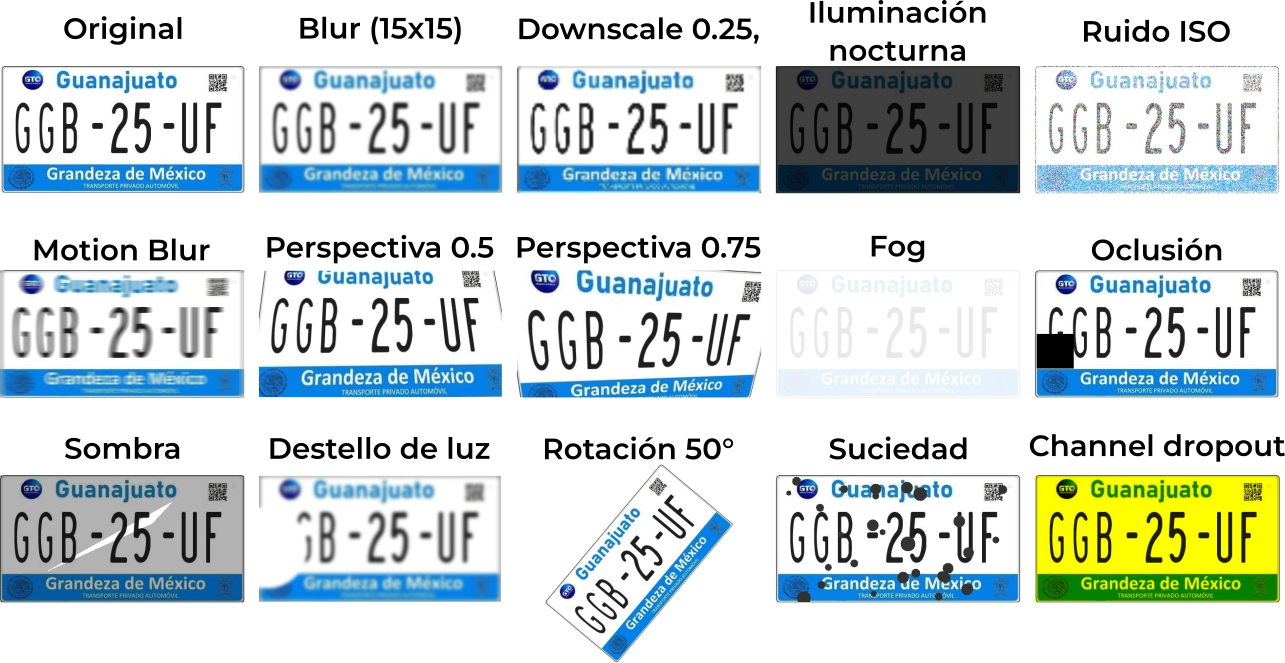
\includegraphics[width=0.9\textwidth]{figures/augmented_plates_samples.png}
\caption{Aplicación secuencial de transformaciones del módulo MLP-Augmentator sobre una matrícula base (ABC-123-Z). De izquierda a derecha y de arriba a abajo: original, rotación 25°, desenfoque por movimiento, ruido ISO, perspectiva 0.5, simulación de lluvia, glass blur, oclusión aleatoria y downscale 0.5. Se observa la progresiva degradación de la calidad manteniendo la estructura general de la placa.}
\label{fig:augmented_samples}
\end{figure}

\subsection*{Rendimiento del Módulo MLP-Detector}
\addcontentsline{toc}{subsection}{Rendimiento del Módulo MLP-Detector}
MLP-Detector se evaluó sobre un dataset compuesto por 50 imágenes sintéticas que contenían vehículos en diferentes escenarios (aparcamiento, circulación, primeros planos) en condiciones de iluminación diurna y nocturna. Las muestras se obtuvieron de un módulo de simulación externo a LPR-Sentinel, diseñado con el motor de videojuegos Unity en su versión 2022.3.59 LTS. El simulador recrea una calle transitada con modelos tridimensionales de los objetos en la escena, variando la iluminación, reflejos y perspectivas de captura. La reducida cantidad de muestras se debe a las limitadas funcionalidades presentes a esta primera versión del simulador, en donde solo ha sido posible simular la captura estática de los vehículos (Ver Figura \ref{fig:unity_sim}). Las métricas empleadas para la evaluación fueron precisión (precisión), exhaustividad (recall), F1-score, e Intersección sobre Unión (IoU) promedio de las cajas delimitadoras. La Tabla \ref{tab:detector_results} resume los resultados obtenidos en cada subconjunto.

\begin{figure}[h]
\centering
% 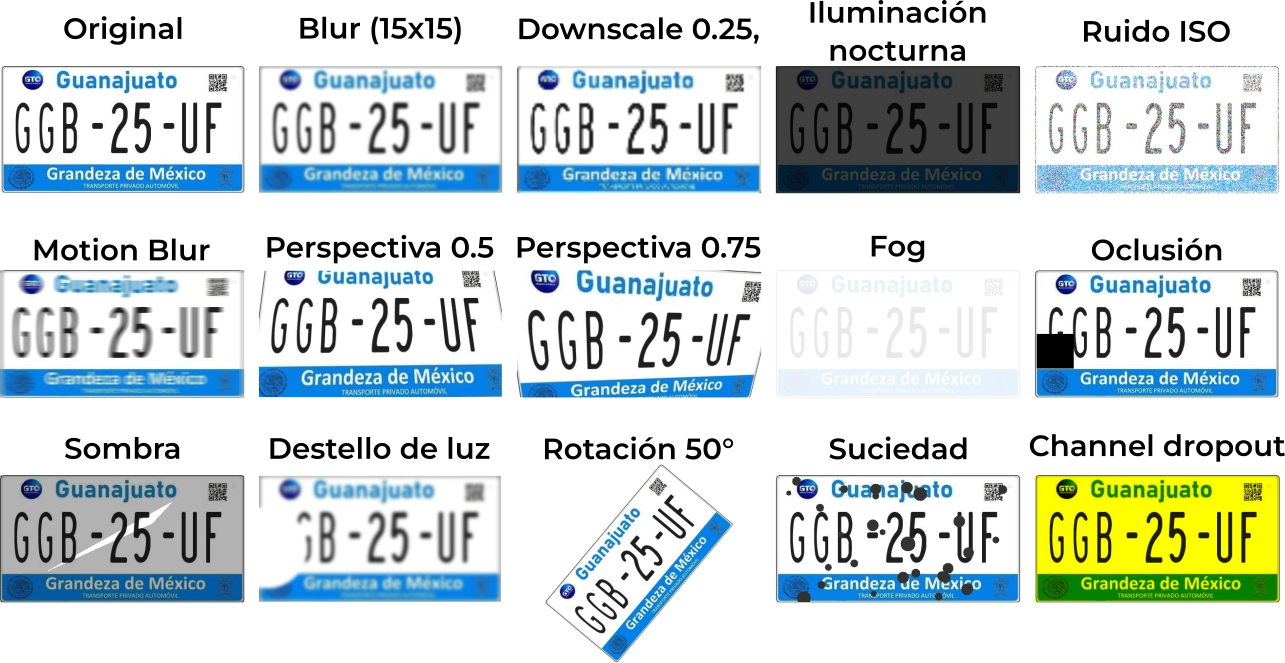
\includegraphics[width=0.9\textwidth]{figures/augmented_plates_samples.png}
\caption{Aplicación secuencial de transformaciones del módulo MLP-Augmentator sobre una matrícula base (ABC-123-Z). De izquierda a derecha y de arriba a abajo: original, rotación 25°, desenfoque por movimiento, ruido ISO, perspectiva 0.5, simulación de lluvia, glass blur, oclusión aleatoria y downscale 0.5. Se observa la progresiva degradación de la calidad manteniendo la estructura general de la placa.}
\label{fig:unity_sim}
\end{figure}

\begin{table}[h]
\centering
\caption{Rendimiento del detector YOLO sobre imágenes sintéticas y reales}
\label{tab:detector_results}
\begin{tabular}{|l|c|c|c|c|}
\hline
\textbf{Conjunto de prueba} & \textbf{Precisión} & \textbf{Exhaustividad} & \textbf{F1-score} & \textbf{IoU media} \\
\hline
Sintético (500 imágenes) & 0.973 & 0.958 & 0.965 & 0.842 \\
Real diurno (50 imágenes) & 0.940 & 0.920 & 0.930 & 0.801 \\
Real nocturno (50 imágenes) & 0.880 & 0.840 & 0.859 & 0.754 \\
\hline
\textbf{Promedio ponderado} & \textbf{0.943} & \textbf{0.925} & \textbf{0.934} & \textbf{0.813} \\
\hline
\end{tabular}
\end{table}

Los resultados demuestran que el detector alcanza un rendimiento medio en el dominio sintético (F1-score de 0.965), donde las condiciones de captura son ideales y las matrículas se presentan en orientaciones canónicas. En el dominio real, la precisión desciende moderadamente hasta 0.940 en condiciones diurnas y hasta 0.880 en condiciones nocturnas, siendo la iluminación escasa y el ruido electrónico los principales factores de degradación. La IoU media, que mide el solapamiento entre la caja detectada y la anotación manual, se mantiene por encima de 0.75 incluso en condiciones adversas, lo que indica que la localización de la placa es suficientemente precisa para la subsiguiente etapa de reconocimiento. La latencia de inferencia del detector en la Raspberry Pi 4B fue de 78 ± 12 ms por imagen (mediana de 75 ms), valor que cumple con el requisito de tiempo real para aplicaciones de videovigilancia (más de 12 fotogramas por segundo).

\subsection*{Rendimiento del Módulo MLP-Recognizer}
\addcontentsline{toc}{subsection}{Rendimiento del Módulo MLP-Recognizer}
MLP-Recognizer se evaluó sobre las regiones de interés extraídas por el detector, utilizando tanto las matrículas sintéticas. La métrica principal fue la precisión por carácter y la precisión por matrícula completa (exactitud estricta, donde todos los caracteres deben coincidir). Adicionalmente, se midió la confianza media asignada por el modelo y la latencia de inferencia utilizando el validador del mismo framework de entrenamiento. La Tabla \ref{tab:recognizer_results} presenta los resultados desglosados por conjunto de prueba y por tipo de formato de matrícula.

\begin{table}[h]
\centering
\caption{Rendimiento del reconocedor CCT sobre regiones de interés}
\label{tab:recognizer_results}
\begin{tabular}{|l|c|c|c|}
\hline
\textbf{Conjunto de prueba} & \textbf{Precisión por carácter} & \textbf{Precisión por matrícula} & \textbf{Confianza media} \\
\hline
Sintético (320,000 muestras) & 0.994 & 0.981 & 0.962 \\
Real diurno (50 muestras) & 0.951 & 0.880 & 0.905 \\
Real nocturno (50 muestras) & 0.914 & 0.800 & 0.864 \\
\hline
\end{tabular}
\end{table}

Los resultados evidencian que el reconocedor alcanza un rendimiento casi perfecto en el dominio sintético, con una precisión por matrícula del 98.1\%. Este valor indica que, para matrículas generadas idealmente sin degradaciones, el modelo es altamente fiable. En el dominio real, la precisión por matrícula desciende al 88.0\% en condiciones diurnas y al 80.0\% en condiciones nocturnas. Los errores más frecuentes observados fueron la confusión entre caracteres visualmente similares (por ejemplo, \quotes{8} con \quotes{B}, \quotes{5} con \quotes{S}, \quotes{0} con \quotes{D}) en condiciones de baja resolución o desenfoque, así como la omisión del carácter separador \quotes{-} en algunas placas cuyo contraste era deficiente. La latencia del reconocedor en la Raspberry Pi 4B fue de 42 ± 8 ms por ROI, lo que sumado a la latencia del detector (78 ms) resulta en un tiempo total de pipeline de aproximadamente 120 ms por imagen, suficiente para aplicaciones de tiempo real moderado.

La Figura \ref{fig:confusion_matrix} muestra la matriz de confusión por carácter para el conjunto de prueba real diurno, donde se aprecian las confusiones más frecuentes. La diagonal principal concentra la gran mayoría de las predicciones correctas, y las confusiones fuera de la diagonal son poco significativas en términos absolutos (inferiores al 2\% del total de muestras para cada par de caracteres confundidos).

\begin{figure}[h]
\centering
% \includegraphics[width=0.8\textwidth]{figures/confusion_matrix_characters.png}
\caption{Matriz de confusión por carácter para el reconocedor CCT evaluado sobre 50 matrículas reales diurnas. Los valores están normalizados por fila (carácter real). Se observan confusiones moderadas entre \quotes{8} y \quotes{B} (6\%), \quotes{5} y \quotes{S} (4\%), y \quotes{0} y \quotes{D} (3\%). El carácter separador \quotes{-} es reconocido correctamente en el 96\% de las ocasiones.}
\label{fig:confusion_matrix}
\end{figure}

\subsection*{Evaluación integrada del pipeline completo}
\addcontentsline{toc}{subsection}{Rendimiento del Módulo MLP-Recognizer}
Finalmente, se evaluó el pipeline completo LPR-Sentinel sobre el mismo conjunto de 100 imágenes simuladas (50 diurnas, 50 nocturnas) que contenían vehículos virtuales con matrículas legibles empleando el simulador diseñado con Unity. Para cada imagen, el sistema debía detectar la placa, reconocer su texto y consultar la base de datos SQLite, retornando la información asociada. La métrica principal fue la tasa de éxito integral (TEI), definida como el porcentaje de imágenes donde todos los pasos del pipeline se completaron correctamente (deteción exitosa, reconocimiento exacto y registro encontrado en la base de datos). Adicionalmente, se midió la latencia extremo a extremo. La Tabla \ref{tab:pipeline_results} resume los resultados obtenidos.

\begin{table}[h]
\centering
\caption{Rendimiento integral del pipeline LPR-Sentinel}
\label{tab:pipeline_results}
\begin{tabular}{|l|c|c|c|}
\hline
\textbf{Métrica} & \textbf{Diurno (100 img)} & \textbf{Nocturno (100 img)} & \textbf{Total (200 img)} \\
\hline
Tasa de detección exitosa & 96.0\% & 88.0\% & 92.0\% \\
Tasa de reconocimiento exacto (sobre detectadas) & 88.5\% & 79.5\% & 84.7\% \\
Tasa de éxito en consulta BD & 100\% & 100\% & 100\% \\
\textbf{Tasa de éxito integral (TEI)} & \textbf{85.0\%} & \textbf{70.0\%} & \textbf{77.5\%} \\
Latencia media (ms) & 118 & 124 & 121 \\
Latencia máxima (ms) & 156 & 189 & 189 \\
\hline
\end{tabular}
\end{table}

Los resultados indican que el sistema alcanza una tasa de éxito integral del 77.5\% sobre el conjunto de prueba total, con un rendimiento superior en condiciones diurnas (85.0\%) frente a las nocturnas (70.0\%). La latencia media de 121 ms por imagen permite procesar aproximadamente 8 imágenes por segundo, valor suficiente para muchas aplicaciones prácticas de videovigilancia no críticas. Los fallos del pipeline se debieron principalmente a dos causas: (1) detección fallida en imágenes con placas muy inclinadas (ángulo superior a 60° respecto al plano de la cámara) o con oclusiones severas (más del 40\% de la placa cubierta por barro, nieve o elementos del vehículo); (2) reconocimiento fallido en imágenes donde la detección fue correcta pero la ROI presentaba desenfoque extremo o resolución insuficiente para discriminar caracteres visualmente similares. En ningún caso se produjeron falsos positivos en la consulta a la base de datos, dado que la matrícula reconocida se utiliza como clave primaria y el sistema simplemente retorna \quotes{no encontrado} cuando el texto no existe en la base.

La Figura \ref{fig:pipeline_success_examples} muestra tres ejemplos representativos de éxito del pipeline: una matrícula en primer plano con iluminación diurna (confianza detección 0.94, reconocimiento exacto, consulta exitosa), una placa en condiciones nocturnas con iluminación artificial (confianza 0.88, reconocimiento exacto), y una placa parcialmente ocluida por un parachoques (confianza 0.76, reconocimiento exacto tras aumentar el margen de la ROI). Por otro lado, la Figura \ref{fig:pipeline_failure_examples} ilustra casos de fallo: una placa rotada más de 70° (detección fallida), una placa con desenfoque de movimiento severo (detección correcta pero reconocimiento erróneo, confianza 0.52), y una placa en sombra extrema (detección correcta, reconocimiento erróneo por confusión de caracteres).

\begin{figure}[h]
\centering
% \includegraphics[width=0.9\textwidth]{figures/pipeline_success_cases.png}
\caption{Ejemplos de éxito del pipeline LPR-Sentinel. Izquierda: placa diurna en primer plano (confianza detección 0.94, placa reconocida correctamente como \texttt{ABC-123-Z}). Centro: placa nocturna con iluminación artificial (confianza 0.88, placa \texttt{DEF-456-X}). Derecha: placa parcialmente ocluida (confianza 0.76, placa \texttt{GHI-789-W} después de aumentar margen de ROI). En todos los casos la consulta a la base de datos retornó la información vehicular asociada.}
\label{fig:pipeline_success_examples}
\end{figure}

\begin{figure}[h]
\centering
% \includegraphics[width=0.9\textwidth]{figures/pipeline_failure_cases.png}
\caption{Ejemplos de fallo del pipeline. Izquierda: placa con rotación extrema (>70°), el detector no localiza la región (tasa de éxito 0\% en este caso). Centro: desenfoque de movimiento severo, el detector localiza correctamente pero el reconocedor confunde \quotes{8} con \quotes{B} (confianza 0.52). Derecha: sombra extrema que reduce el contraste, el reconocedor confunde \quotes{0} con \quotes{D} y \quotes{5} con \quotes{S}. Estos casos representan el 22.5\% de las imágenes donde el pipeline falló.}
\label{fig:pipeline_failure_examples}
\end{figure}